%-*-latex-*-
\tinysidebar{\debug{exercises/discrete-probability/{bernoulli-05/answer.tex}}}

The probability of getting at least 2 sixes is
\[
B(n,p; 2) + 
B(n,p; 3) + 
B(n,p; 4) + 
\cdots + 
B(n,p; 7) 
\]
Therefore the student will earn
\[
\left(
  B(n,p; 2) + 
  B(n,p; 3) + 
  B(n,p; 4) + 
  \cdots + 
  B(n,p; 7)
  \right) \times 100 - 1
\]
(The \lq\lq $-1$'' is because the student has to pay \$1 to play.) 
Of course to make money, you will want
\[
\left(
  B(n,p; 2) + 
  B(n,p; 3) + 
  B(n,p; 4) + 
  \cdots + 
  B(n,p; 7)
  \right) \times 100 - 1 < 0
\]
i.e.,
\[
  B(n,p; 2) + 
  B(n,p; 3) + 
  B(n,p; 4) + 
  \cdots + 
  B(n,p; 7)  < 1/100
\]
It's easier to use this:
\[
  1
  - B(n,p; 0) 
  - B(n,p; 1) 
  - B(n,p; 2) 
  < 1/100
\]
and therefore we want
\[
  99/100 < B(n,p; 0) + B(n,p; 1) + B(n,p; 2)
\]
which is the same as
\[
99/100
<
\binom{7}{0}p^0(1-p)^{7-0}
+
\binom{7}{1}p^1(1-p)^{7-1}
+
\binom{7}{2}p^2(1-p)^{7-2}
\]

The following is a graph for different values of $p$:
%-*-latex-*-

\begin{center}
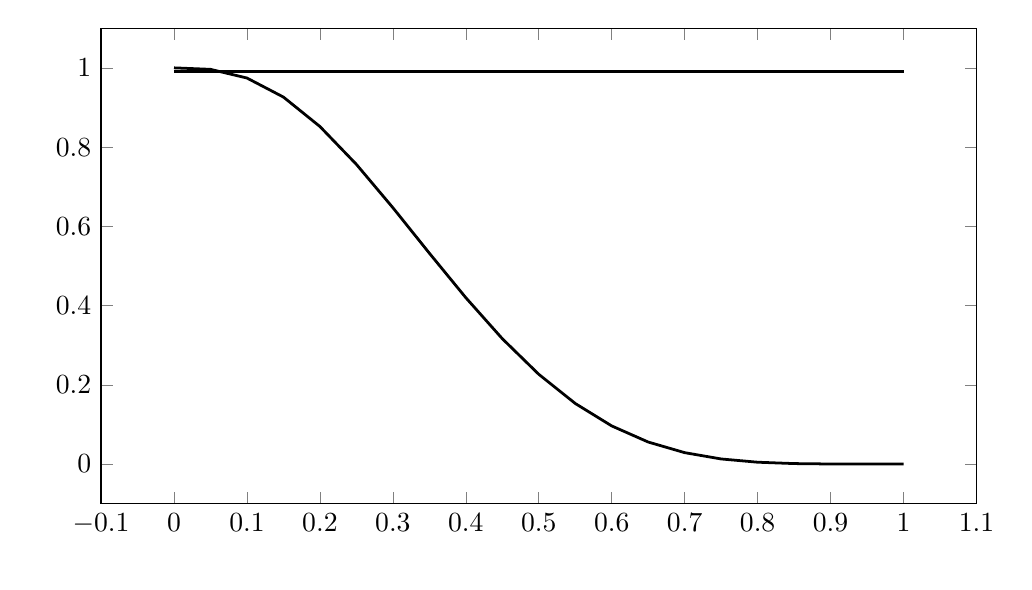
\begin{tikzpicture}[line width=1]
\begin{axis}[width=5in, height=3in,
             scatter/classes={a={mark=*,draw=black}},
             xlabel={\mbox{}},
             xlabel style={name=xlabel}, 
             ylabel={\mbox{}}, 
             legend style={
                at={(xlabel.south)},
                yshift=-1ex,
                anchor=north,
                legend cell align=left,
                },
        ]
]
\addplot[draw=black, line width=1] coordinates {(0.0, 1.0)
(0.05, 0.9962429570312497)
(0.1, 0.9743085000000002)
(0.15, 0.9262348398437498)
(0.2, 0.8519680000000004)
(0.25, 0.75640869140625)
(0.3, 0.6470694999999997)
(0.35, 0.53228332421875)
(0.4, 0.41990399999999994)
(0.45, 0.31644005078125015)
(0.5, 0.2265625)
(0.55, 0.15292768359374995)
(0.6, 0.09625600000000004)
(0.65, 0.055607535156249985)
(0.7, 0.02879550000000002)
(0.75, 0.01287841796875)
(0.8, 0.004671999999999996)
(0.85, 0.0012216445312500006)
(0.9, 0.00017649999999999982)
(0.95, 6.0273437500000275e-06)
(1.0, 0.0)};\addplot[draw=black, line width=1] coordinates {(0.0, 0.99)
(0.05, 0.99)
(0.1, 0.99)
(0.15, 0.99)
(0.2, 0.99)
(0.25, 0.99)
(0.3, 0.99)
(0.35, 0.99)
(0.4, 0.99)
(0.45, 0.99)
(0.5, 0.99)
(0.55, 0.99)
(0.6, 0.99)
(0.65, 0.99)
(0.7, 0.99)
(0.75, 0.99)
(0.8, 0.99)
(0.85, 0.99)
(0.9, 0.99)
(0.95, 0.99)
(1.0, 0.99)};
\end{axis}\end{tikzpicture}\end{center}

Zooming in on the part of the graph where $x$ is in $[0.05, 0.1]$, we get
%\begin{python}
%from math import *
%from latextool_basic import *
%plot = FunctionPlot(width="7in")
%
%import scipy.misc
%comb = scipy.misc.comb
%
%def B(n, p, k):
%    return comb(n, k) * p**k * (1-p)**(n - k)
%
%def f(p):
%    return B(7, p, 0) + B(7, p, 1) + B(7, p, 2)
%
%myrange = [0.05, 0.06, 0.08, 0.1]
%data1 = [(i,f(i)) for i in myrange]
%data2 = [(i,0.99) for i in myrange]
%
%plot.add(data1, line_width='1', color='black')
%plot.add(data2, line_width='1', color='black')
%print(plot)
%\end{python}

\begin{center}
\begin{tikzpicture}[line width=1]
\begin{axis}[width=5in, height=3in,
             xlabel={\mbox{}},
             xlabel style={name=xlabel}, 
             ylabel={\mbox{}},
             xtick=data,
             yticklabels={,,},
             tick label style={/pgf/number format/fixed},
             legend style={
                at={(xlabel.south)},
                yshift=-1ex,
                anchor=north,
                legend cell align=left,
                },
        ]
]
\addplot[draw=black, line width=1] coordinates
 {(0.05, 0.996)
  (0.06, 0.994)
  (0.08, 0.986)
  (0.10, 0.974)};
\addplot[draw=black, line width=1] coordinates
 {(0.05, 0.990)
  (0.06, 0.990)
  (0.08, 0.990)
  (0.10, 0.990)};
\end{axis}
\end{tikzpicture}\end{center}

Therefore the break even value for $p$ is approximately $0.07$.
(For a fair die, the probability for getting a six is $1/6 = 0.167$.)

We now compute our gains for a few values of $p$ near $0.07$.
If $p = 0.06$, then the player would make
\[
(1 - B(7,0.06;0) - B(7,0.06;1) - B(7,0.06;2)) \times 100 - 1
=
-0.3706...
\]
which means that we gain \$0.37 per game.
If $p = 0.07$, then the player would make
\[
(1 - B(7,0.07;0) - B(7,0.07;1) - B(7,0.07;2)) \times 100 - 1
=
-0.0312...
\]
which means that we gain \$0.03 per game.
If $p = 0.08$, then the player would make
\[
(1 - B(7,0.08;0) - B(7,0.08;1) - B(7,0.08;2)) \times 100 - 1
= 0.4014....
\]
which means that we would lose \$0.40 per game.

So, for instance, if we use $p = 0.07$ and a total of 100 games were
played, we will collect \$37.00.




[TO TIDY UP]
